%************************************************
\chapter{Discussion}
\label{chp:Discussion}
%************************************************
%\section{Parallel processing streams and their functional significance}
%Parallel processing seems to be a successful evolutionary strategy conserved throughout phyla. Other than the visual system, the olfactory system of the nematode C elegans \parencite{Chalasani2007} and the auditory cortex of mammals \parencite{Scholl2010} are some examples where parallel circuits compute ON and OFF signals separately.
In manuscript \ref{sct:manuscript_haag_mishra}, we found that the elementary motion-sensitive neurons T4 and T5 in \textit{Drosophila} regardless of their directional tuning and contrast preferences for ON or OFF stimuli implemented a preferred direction (PD) enhancement on the preferred side of their receptive field and a null direction (ND) suppression on the null side. This combination of PD enhancement and ND suppression increases the direction selectivity in T4 and T5 cells, the first cells where the direction selectivity emerges. In T4 cells, whole-cell patch clamp recordings revealed that while the preferred direction stimuli led to large membrane depolarizations, the null direction stimuli also evoked small, but significant responses \parencite{Groschner2022}. The calcium recordings, however, had a large response to stimuli moving in the preferred direction and almost no response to stimuli moving in the null direction \parencite{Maisak2013, Fisher2015}. In manuscript \ref{sct:manuscript_mishra_haag}, we showed that the voltage-to-calcium transformation in addition to the synaptic mechanisms on the dendrites of the T4 neurons enhances the direction selectivity in the T4 neurons: the calcium signals in T4 cells had a significantly higher direction selectivity compared to the voltage signals, thus making T4 output signals more direction-selective.  

\section{Cellular implementation of motion vision}
How are PD enhancement and ND suppression implemented in T4 and T5 cells?  Through decades of research, a complete connectome of motion vision circuitry has been assembled \parencite{Takemura2008, Takemura2017, Shinomiya2014, Shinomiya2019}. A great deal of detail has been provided on the functional response properties \parencite{Arenz2017, Drews2020, Strother2017, Serbe2016} and transmitter phenotypes \parencite{Davis2020, Pankova2017, Richter2018, Takemura2017} of the inputs to T4/T5 cells. Furthermore, it is also possible to visualize the endogenous expression of receptor proteins in T4 and T5 neurons. The subcellular distributions of the Acetylcholine (ACh) receptor subunit \textit{D$\alpha$7}, the GABA receptor subunit \textit{Rdl}, and the glutamate-gated chloride channel \textit{$GluCl\alpha$} have been studied in T4 and T5 cells \parencite{Fendl2020}.

In the T4 dendrites, \textit{$GluCl\alpha$} receptors and the glutamatergic input Mi9 synapses are located on the distal part (the preferred side) of the dendrite (figure \ref{fig:receptors}c, e). The ACh \textit{D$\alpha$7} receptors and the cholinergic inputs Mi1 and Tm3 synapses are located at the center of the T4 dendrites. The GABA Rdl receptors and the GABAergic inputs Mi4, C3, and CT1 synapses are located on the proximal (the null side) of the T4 dendrites. The presence of the glutamate-gated chloride channels makes glutamate input from Mi9 inhibitory. Mi9 has an OFF center receptive field. Mi9 maintains an active state in the dark that abruptly ends when light stimulates its receptive field. The preferred direction enhancement or the multiplication-like nonlinearity arises from the coincidence of cholinergic excitation and release from glutamatergic inhibition \parencite{Groschner2022}. The PD enhancement on the T4 dendrites is thus achieved by multiplying the release from Mi9 inhibitory glutamate input on the distal arm with an excitatory cholinergic input of Mi1 in the center. This 'multiplicative disinhibition' represents the opposite of divisive inhibition. GABAergic inhibitory inputs on the null sides Mi4, C3, and CT1 provide the divisive inhibition or the null direction suppression. Why are there multiple cells providing input on the null side and the specific contributions of each of these cells on the null side remain to be investigated.

There is still uncertainty regarding how PD enhancement and ND suppression are achieved in T5 dendrites. In the T5 dendrites, the ACh \textit{D$\alpha$7} receptors and the cholinergic Tm1, Tm2, and Tm4 inputs synapses are located in the center of the dendrites (figure \ref{fig:receptors}d, f). The GABA \textit{Rdl} receptors and the GABAergic input CT1 synapses are located on the proximal part (the null side) of the dendrites. However, the \textit{$GluCl\alpha$} receptors are absent in the case of T5 cells. The T5 dendrites on the distal part (the preferred side) receive input from cholinergic neuron Tm9 and also express ACh receptors. Hence, the implementation of PD enhancement in the case of T5 cells is most likely different from the implementation in the T4 cells. In addition, while 3 neurons (Mi4, C3, and CT1) provide GABAergic input to the null side of T4 dendrites, the T5 neurons receive inhibitory input on the null side only from CT1 neurons. As a result of these differences, the implementation of ND suppression in T5 cells may also be different in comparison to the T4 cells. These are some of the questions that need to be investigated further. 

One possible approach to discern the individual contribution of the GABA-ergric input neurons Mi4, C3, and CT1 is to silence one of these neurons, while simultaneously recording neural activity from the T4 neurons. However, such blocking experiments come together with their own challenges. One such challenge is that the current blocking techniques are not connection-specific. In other words, silencing one type of cell will silence synaptic transmission to all of its postsynaptic targets. Especially in the fly visual system, where almost all of the medulla neurons are highly interconnected, this can be problematic \parencite{Takemura2017}. For example, Mi4 and Mi9 cells have very strong reciprocal connections. Hence, silencing Mi4 neurons would also affect the neural activity in the Mi9 neurons. The effect thus observed downstream in T4 neurons is difficult to be attributed solely to Mi4. It is therefore possible to cause second-order effects if one cell type is blocked, resulting in a profound effect on the circuit overall. The development of connection-specific blockers could provide a solution to such confounding effects. Secondly, it is difficult to determine the effectiveness of a block. It is hard to say whether blocked cells have no effect or if the block was ineffective when there is no effect or negative results. Thirdly, does the stimulus being used test the distinct contribution of the cell to the response? If no effect or phenotype is observed and the block is effective, using another stimulus may result in an effect.

\begin{figure}
\centering
\hspace*{-1cm} 
\includegraphics[scale=0.8]{Receptors_Fig_1}
\caption[Distribution of the presynaptic partners, input synapses and receptors on the T4 and T5 dendrites] {Distribution of the presynaptic partners, input synapses and receptors on the T4 and T5 dendrites: (a) A horizontal view of the optic lobe shows the retina, lamina, medulla, lobula, and lobula plate. Dendrites of T4 (darker gray) are found in layer 10 of the medulla, and those of T5 (lighter gray) are found in layer 1 of the lobula. (b) An EM-reconstructed T4 neuron showing the location of the dendrite, axon, and cell body. (c) An illustration of an individual T4 dendrite and its distribution of input synapses (frontal view). In this illustration, the dendrite points to the right, against its preferred right-to-left orientation (indicated by an arrow). (d) Same as in c, but for T5 cells. (e) Anatomic distribution of glutamate-gated chloride channels \textit{$GluCl\alpha$}, acetylcholine receptors \textit{D$\alpha$7}, and GABA receptors \textit{Rdl} on T4 dendrites. (f) Same as in e, but for T5 cells. (Used and modified with permission from \parencite{Fendl2020})} 
\label{fig:receptors}
\end{figure}

\subsection{Mechanism for the temporal delay}
Most major cells presynaptic to T4 and T5 have been characterized in detail in terms of their temporal response properties. Generally, inputs can be classified into two classes with respect to their temporal properties: transient band-pass filters and slow sustained low-pass filters \parencite{Arenz2017, Serbe2016, Behnia2014}. In the ON pathway, while Mi9 and Mi4 show characteristics of a low-pass filter, Mi1 and Tm3 show characteristics of a band-pass filter. In the OFF pathway, Tm1, Tm2, and Tm4 revealed a band-pass characteristic, and Tm9 showed low-pass filter characteristics. The mechanisms underlying their diverse temporal properties, however, remain unknown. It is possible to implement a delay either intracellularly or synaptically. Simple mechanisms such as passive dendritic filtering can be used by cells. A neurite's length, diameter, and membrane resistance, for example, determine its conduction velocity. The time constant of a neuron, which describes its passive low-pass filtering properties, is linearly related to its input resistance. Therefore, slower medulla neurons may simply have higher resistances.

In addition to the cellular passive properties, voltage-gated ion channels can also delay electrical signals or render them more transient \parencite{Destexhe1999}. As an example, depolarizing synaptic inputs activate A-type potassium channels, but they quickly deactivate. The brief increase in potassium conductance prevents the membrane from reaching a threshold, causing a delay \parencite{Groschner2018}. In the lateral geniculate nucleus of guinea pigs, a transient A-type potassium current has been hypothesized to explain the delayed visual response \parencite{Mccormick1991}.

Synaptic transmission can have an important impact on a circuit's temporal dynamics in addition to cell-intrinsic mechanisms. The process of neurotransmitter release, diffusion, and binding to a receptor already imposes a delay of 2-3 milliseconds during chemical synaptic transmission. Additionally, postsynaptic receptor properties contribute to temporal filtering. Direct current can flow through ionotropic receptors, but metabotropic receptors initiate a second messenger cascade, which activates ionic conductances after a delay typically of tens to hundreds of milliseconds. All of these mechanisms are plausible since T4 and T5 neurons express a wide array of ionotropic and metabotropic neurotransmitter receptors and voltage-gated ion channels. 

Mi9 and Tm9 with low-pass filter characteristics receive their major input from lamina cell L3, which exhibits slow temporal characteristics \parencite{Silies2013}. L1 provides a major input to the faster cells Mi1 and Tm3 \parencite{Takemura2017}. There are already fast band-pass characteristics in L1 \parencite{Clark2011, Reiff2010, Drews2020}. Therefore, it is possible that medulla neurons inherit the temporal properties of their lamina inputs. Thus, the delay mechanism associated with ON and OFF motion detectors may be implemented between photoreceptors and lamina cells at the first synapse. In this scenario, motion blindness should be the result of flies with dysfunctional L3 cells. However, blocking synaptic transmission from L3 does not significantly affect fly optomotor activity \parencite{Bahl2015, Silies2013, Tuthill2013}. The temporal filtering properties of a given neuron in the fly medulla are likely determined by several biophysical mechanisms.

 
%\section{Neural correlates implementing direction selectivity in the ON and the OFF pathways}
%We found that elementary motion-sensitive neurons T4 and T5 in \textit{Drosophila} regardless of their directional tuning and contrast preferences for ON or OFF stimuli implement a preferred direction enhancement on the preferred side of their receptive field and a null direction suppression on the null side. The presynaptic cells for T4 cells are Mi1, Tm3, TmY15, Mi4, Mi9, C3, and CT1. The presynaptic cells for T5 cells are Tm1, Tm2, Tm4, TmY15, Tm9, CT1, LT33, and Tm23. Moreover, each subtype of a T4 cell receives synaptic input from another T4 cell of the same type. For T5 cells, the same applies. 
%
%Blocking Mi1 completely abolished responses to ON edges, and blocking Tm3 mostly affected responses at high speeds \parencite{Ammer2015}. Therefore, Tm3 seems to be specifically needed to detect the direction of ON edges at high velocities. Mi1 provides excitatory cholinergic inputs to the central part of T4 dendrites. Mi9 provides inhibitory glutamatergic inputs to the preferred side of T4 dendrites. The preferred direction enhancement or the multiplication-like nonlinearity arises from the coincidence of cholinergic excitation and release from glutamatergic inhibition \parencite{Groschner2022}. This 'multiplicative disinhibition' represents the opposite of divisive inhibition. GABAergic inhibitory inputs on the null sides Mi4, C3, and CT1 provide the divisive inhibition or the null direction suppression. Why are there multiple cells providing input on the null side and the specific contributions of each of these cells on the null side remain to be investigated.
%
%In the OFF pathway, selectively blocking individual Tm cells or combinations of them resulted in a range of effects on gratings and edge responses. However, no specific stimulus space could be identified where the contributions of different cells could be segregated \parencite{Serbe2016}. Tm1, Tm2, Tm4, and Tm9 provide excitatory cholinergic inputs on T5 dendrites. How is preferred direction enhancement implemented in T5 cells, with a cholinergic input on the preferred side? CT1 is the only GABAergic input providing inhibition on the null side of T5 dendrites. Does CT1 provide null direction suppression to the T5 dendrites? Why are there 3 cells providing inhibitory input on the null side of T4 dendrites compared to 1 cell providing inhibitory input on the null side of T5 dendrites? These questions are still being investigated in the OFF pathway. 

\subsection{Circuits downstream of T4 and T5 cells}
How do downstream circuits use the motion direction information computed by the T4/T5 neurons in the optic lobe to guide fly behavior? The crucial roles of T4 and T5 cells in visually guided behaviors have been revealed through several studies inhibiting synaptic transmission from these cells. For fly optomotor behavior, T4 and T5 cells are required. Blocking the synaptic output of these cells led to motion blindness in flies \parencite{Bahl2013}. Figure-ground discrimination \parencite{Fenk2014}, avoidance of expanding stimuli, as well as landing responses \parencite{Schilling2015} involve T4 and T5 cells. In what ways are direction-selective signals passed from T4/T5 cells to the central brain and to the motor areas? Lobula plate tangential cells (LPTCs) provide the most direct link between motion-sensitive T4/T5 neurons and motor circuits. 

In the lobula plate, T4 and T5 neurons provide excitatory inputs onto LPTCs and lobula plate intrinsic neurons (Lpi). In addition to abolishing the depolarization of LPTCs when stimulated along their preferred direction, blocking the output of T4 and T5 cells also affects the hyperpolarization when stimulated along their null direction \parencite{Schnell2012}. Additionally, LPTCs respond with a fast excitation, followed by inhibition when T4 and T5 are optically activated \parencite{Mauss2015}. These results suggest that T4 and T5 cells provide LPTCs with both direct stimulation and indirect inhibition from adjacent lobula plate layers. Since LPi neurons bi-stratify in layer-specific ways, dendrites from one subtype reside exclusively in one layer, and axons in the neighboring layer, LPi are perfect candidates for this task (figure \ref{fig:lpifigure}). T4/T5 cells in one layer provide feedforward glutamatergic inhibitory input via LPi via glutamate-gated chloride channels \textit{$GluCl\alpha$} to LPTC dendrites in the adjacent layer. The LPis are thus essential for increasing flow-field selectivity since it subtracts motion-opponent signals \parencite{Mauss2015}.

%Dendritic trees of the LPTCs span large areas of the lobula plate, sometimes even covering the entire layer. They, therefore, cover a large portion of the visual field with their receptive fields. There are two major groups of Drosophila's LPTCs, based on their response characteristics: The horizontal system (HS) and the vertical system (VS) cells. When presented with motion in a preferred direction (PD), LPTCs depolarize, while when presented with motion in a null direction (ND), they hyperpolarize. The T4 and T5 excitatory inputs from one lobula plate layer are integrated and subtracted from the adjacent layer. Dendrite location determines the preferred direction. As all preferred directions are combined onto the dendritic tree, so-called flow fields emerge that describe the optimal pattern of motion resulting from ego-motion. Thus, LPTCs are specialized filters that detect optical flow patterns resulting from self-motion \parencite{Krapp1996}. During the tethered flight, unilateral activation of HS cells induces yaw-turning responses of the head and wings \parencite{Haikala2013}. VS and HS synaptic output blocks impair the head optomotor response severely but have a weaker impact on wing steering \parencite{Kim2017}. Accordingly, \textit{Drosophila} optomotor responses may be controlled by LPTCs.

\begin{figure}
\centering
\hspace*{-1cm} 
\includegraphics[scale=0.7]{LPi_figure}
\caption[Lobula plate intrinsic neurons (LPis)] {Lobula plate intrinsic neurons (LPis): (a) Multi-color flip-out showing several LPi neurons in the lobula plate. D = dorsal, V = ventral, L = lateral, M = medial. (b) Dendritic fields of adjacent LPi neurons shown schematically. (c) The horizontal cross-section of the lobula plate shows GFP-expressing T4/T5 cells (green) and synaptotagmin-HA (red). (d) LPi neurons expressing GFP (green) and presynaptic synaptotagmin-HA (sytHA, red). Presynaptic specializations are restricted to layer 4 only, even though neurons ramify in layers 3 and 4. (e) GFP staining of a VS cell dendrite in layer 4 of the lobula plate. (f) Patch-clamp recordings from VS cells and optogenetic stimulation of LPi cells to study the synaptic connection between LPi and VS cells. A sustained hyperpolarizing potential is evoked by 1 s light stimulation of LPi neurons (upper recording trace). Light pulses (2 ms) are delivered in different strengths (bottom traces). (g) Direction-selectivity of Lpi cells. Visual activity in LPi3-4 neurons measured by calcium imaging in response to gratings moving in different directions. (Used with permission from \parencite{Borst2020b})} 
\label{fig:lpifigure}
\end{figure}


%\subsection{Direction selectivity of T4 output signals}
%In addition to the dendritic integration of postsynaptic voltages or after the action potential is generated, further computations can occur in the transformation between voltage and calcium, or between calcium and neurotransmitter release. Neuronal signaling and information processing involves the transformation of membrane voltage into calcium signals, which lead to transmitter release. 
%In our second manuscript \ref{sct:manuscript_mishra_haag}, 
We showed that the voltage to calcium transformation in T4c neurons enhances their direction selectivity. The calcium signals in T4c cells had a significantly higher direction selectivity and tuning than the membrane voltage across different stimuli conditions. As calcium is required for neurotransmitter release, this is expected to increase the direction selectivity of T4 cells' output signals. In order to determine the direction selectivity of T4 cells' output signals, the neurons that are postsynaptic to T4 cells can be recorded. As discussed, the HS cells with dendrites in layer 1 depolarize during front-to-back motion and hyperpolarize during back-to-front motion, while HS cells in layer 2 display the opposite tuning, while VS cells with dendrites mainly in layer 4 depolarize primarily during downward motion and hyperpolarize during upward motion \parencite{Schnell2010, Hopp2014, Scott2002}. Monosynaptic, excitatory, and cholinergic connections exist between T4/T5 and tangential cells \parencite{Mauss2014}. T4/T5 cells are responsible for depolarizing tangential cells during preferred direction motion. Tangential cells hyperpolarise in the null direction in response to inhibition from Lpi neurons, which receive excitatory input from T4/T5 neurons in the opposite layer. Upon silencing the LPi3-4 neurons’ synaptic output via tetanus toxin, the VS neurons' depolarization response in the preferred direction did not change, but the null direction response was absent (figure \ref{fig:lpiblock}) \parencite{Mauss2015}. This suggests T4/T5 do not release any transmitter in response to the null direction motion, which matches our findings for the calcium responses. Thus, the voltage to calcium transformation increases direction selectivity in T4/T5 cells and this enhances direction selectivity in the downstream neurons.
%The direction selectivity index for calcium signals compared with voltage signals for a few stimuli conditions was previously found to be higher in a study in T5 cells using ASAP2f as an optical voltage indicator \parencite{Wienecke2018}. How does this affect the output signal of T4/T5 neurons?

%As calcium is required for neurotransmitter release, this is expected to increase the direction selectivity of T4/T5 cells' output signals. In the lobula plate, the T4/T5 cells provide inputs onto large lobula plate tangential cells that are depolarized during preferred and hyperpolarized during null direction motion \parencite{Mauss2014}. For example, the vertical system (VS) cells with dendrites in layer 4 receive direct excitatory inputs from downward tuned T4d/T5d neurons causing depolarization during motion in the downward preferred direction. These VS cells also receive indirect inhibitory inputs from upward tuned T4c/T5c neurons via the glutamatergic LPi3-4 neurons projecting from layer 3 to layer 4 causing hyperpolarization in VS cells during motion in the upward null direction. 


\begin{figure}
\centering
\hspace*{-1cm} 
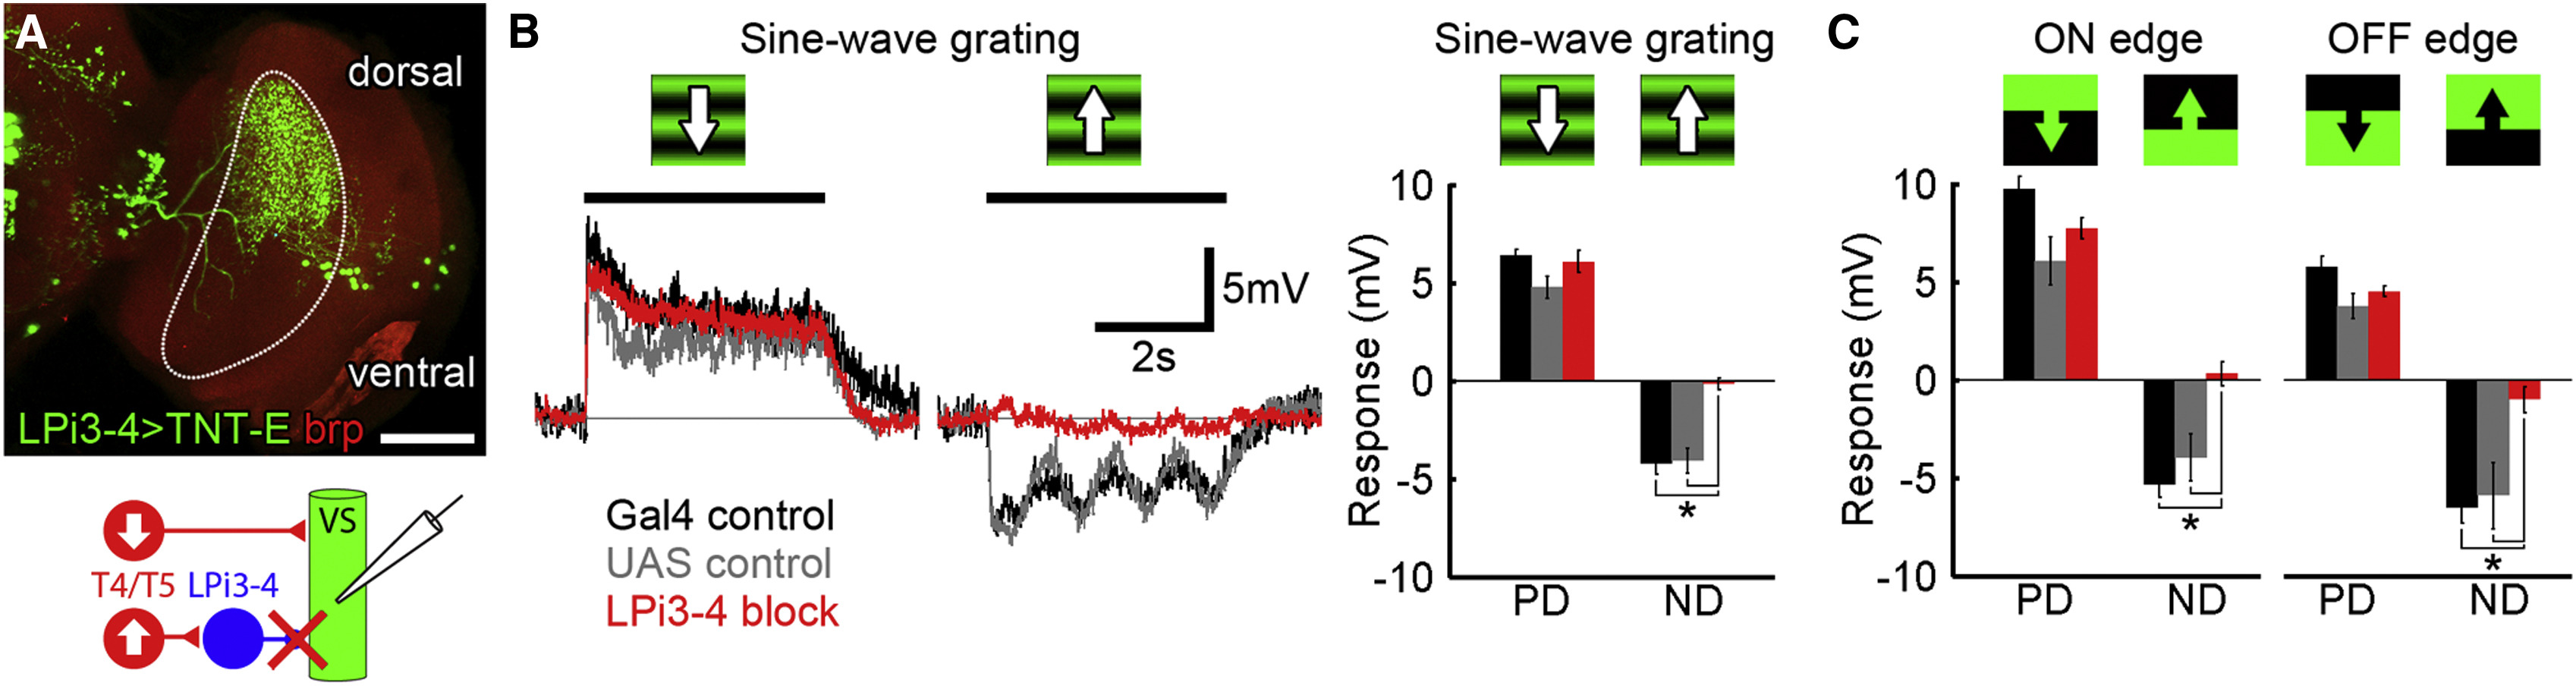
\includegraphics[scale=0.8]{LpiBlock}
\caption[Tangential cells receive null direction responses from LPi neurons] {Tangential cells receive null direction responses from LPi neurons: (a) In LPi3-4 neurons, the tetanus toxin light chain suppresses synaptic release. The schematic below illustrates the experimental approach used to measure whole-cell voltages from VS cells in order to investigate LPi3-4 cell function. (b) Control flies respond to sine-wave gratings moving down (preferred direction [PD]) or up (null direction [ND]) by depolarizing or hyperpolarizing respectively. Hyperpolarizing responses to ND motion are selectively abolished in LPi3-4 block flies. (c) In LPi3-4 block flies, VS cell responses to moving ON and OFF edges are similarly affected with ND responses. (Used with permission from \parencite{Mauss2015})} 
\label{fig:lpiblock}
\end{figure}

\section{The function of the visual circuit during natural behavior}
In this thesis, experiments were conducted on tethered flies whose movement is severely restricted. How do motion circuits operate during unrestrained behavior? State-dependent modulations are observed in the activity and tuning properties of visual circuits in mice and flies \parencite{Maimon2011}. During tethered flight or walking, tangential cells in the fly's lobula plate shift their temporal frequency tuning optimum towards higher frequencies \parencite{Chiappe2010, Maimon2010, Jung2011}. In the ON motion vision pathway, the medulla neurons modulate their baseline calcium level according to their behavioral state, and octopaminergic neurons are needed to process fast-moving visual stimuli appropriately \parencite{Strother2018}. Chlordimeform (CDM), an octopamine agonist, shifted the temporal tuning optima for T4 and T5 cells and all input elements towards higher frequencies \parencite{Arenz2017}. Both mammalian and fly visual systems are affected by the general behavior state of the animal early on in the circuit and only a few synapses from photoreceptors.

A free-moving or flying fly experiences not only visual cues but also proprioceptive cues through its antennae and halteres \parencite{Mamiya2011, Sandeman1980}. Multiple cues are combined in higher multimodal circuits, usually in a non-linear way \parencite{Haag2010, Huston2009}. As a result, the activity of visually responsive neurons during tethered flight might be completely different from that during free flight. Flies perform complex maneuvers during free flight, often involving multiple axes of rotation and translation. In a restrained environment, these maneuvers are hard or impossible to repeat. In order to fully understand the function of a visual circuit, it is ideally best to study it in its natural state. In larger animals that can carry head-mounted microscopes, head-stages, or fiber optics, this is easier, but in fruit flies, it is extremely challenging. Over the past years, substantial progress has been made toward achieving this goal. Fruit flies can be tracked online in 2D and 3D with high precision. An optical laser can be used to target the fly for thermogenetic or optogenetic activation of nerve cells using this information \parencite{Bath2014, Stowers2014, Straw2011}. It is therefore possible to manipulate the activity of a subset of neurons when a fly performs a specific behavioral action or experiences a visual stimulus. Efforts are being made to perform functional imaging in freely walking flies \parencite{Grover2016}. The combined use of these promising tools can give us a better understanding of how individual nerve cells and visual circuits operate under natural conditions.

\section{Comparison with the direction-selective circuits in the mouse retina}
Among the most striking similarities between the retina and the fly optic lobe is the early splitting of pathways into ON and OFF channels (figure \ref{fig:flymouse}). This allows for more efficient encoding of visual stimuli \parencite{Gjorgjieva2014}. In the vertebrate retina, this splitting takes place right at the photoreceptor-bipolar synapse, whereas in the fly, it occurs one synapse later.

The photoreceptors of the mouse retina hyperpolarize in response to light, while in darkness they release glutamate onto their postsynaptic partners, the bipolar cells. The split between the ON and OFF pathways occurs at the synaptic level between photoreceptors and bipolar cells, resulting in the ON- and OFF-responsive bipolar cells. In the ON bipolar cells, the metabotropic inhibitory glutamate receptor mGluR6 causes a sign inversion and the ON channel is formed \parencite{Masu1995}. The OFF bipolar cells, however, express ionotropic AMPA receptors that depolarize when glutamate binds \parencite{Euler2014}. As in the fly optic lobe, there are fast and slow bipolar cells, similar to the medulla and transmedulla neurons.

In the fly, the split into the ON and OFF pathways occurs at the level of lamina cells. Vertebrates don't seem to have any equivalent to the lamina. The \textit{Drosophila} photoreceptors depolarize under light and release histamine, which in turn inhibits lamina neurons via histamine-gated chloride channels \parencite{Hardie1989}. The cholinergic lamina neurons L2-L5 transmit photoreceptor signals to the medulla and transmedulla neurons. In the ON channel, L1 is the main input, while in the OFF channel, L2 is the main input \parencite{Joesch2010}. The glutamatergic L1 neurons inhibit postsynaptic Mi1 and Tm3 neurons via the glutamate-gated chloride channel GluCl$\alpha$, implementing a sign inversion and creating an ON channel. Thus, the photoreceptors depolarize in response to the light, inhibiting L1 neurons, thereby disinhibiting Mi1 and Tm3 neurons, creating the ON-responses. Both GluCl$\alpha$ and Rdl receptors are involved in this multi-synaptic sign inversion in the ON pathway \parencite{Molina2019}. Both mouse and fly visual systems exhibit sign inversion in the ON pathway as a result of glutamatergic, inhibitory signaling. Fly uses the GluCl$\alpha$ channel, which is unique to the invertebrates, instead of the mGluR6 receptor, which causes inhibition in the mouse retina.

Direction-selective T4/T5 cells in the flies are comparable to the starburst amacrine cells (SACs) in mammals and the lobula plate tangential cells are comparable to direction-selective ganglion cells (figure \ref{fig:flymouse}). The direction-selective retinal ganglion cells (DSGCs) were the first direction-selective cells to be described in the mammalian retina \parencite{Barlow1963}. Their four subtypes respond to movement in one of the four cardinal directions, similar to the elementary motion detectors in the fly (T4/T5 neurons) \parencite{Elstrott2008}. Pharmacology and ablation experiments suggest that GABAergic starburst amacrine cells (SACs) are necessary for direction-selective responses in retinal ganglion cells \parencite{Yoshida2001}. It is interesting to note that starburst amacrine cells are already direction-selective themselves in a centrifugal manner \parencite{Euler2002}. Dendrites of these cells protrude radially, and they respond preferentially to stimuli from the base to the tip of the cell. The SACs, in turn, enable DSGCs to be direction selective by inhibiting the null side of their dendrites with asymmetric GABAergic inhibition \parencite{Briggman2011}. How do the SACs become direction-selective? There are several hypotheses and lines of evidence about how bipolar cells providing excitatory glutamatergic input to both cell types shape their direction-selective responses. The starburst amacrine cells which respond to stimuli moving from the soma to the dendritic tips receive input from different types of bipolar cells, including those with fast and slow temporal dynamics \parencite{Baden2013}. The different types of bipolar cells also exhibit space-time wiring specificity with starburst amacrine cells: slow bipolar cells wire with starburst amacrine cells proximally, whereas fast bipolar cells wire with the starburst amacrine cells distally \parencite{Kim2014}. Thus, direction selectivity in flies and mammals may arise by similar mechanisms.

\begin{figure}
\centering
\hspace*{-1cm} 
\includegraphics[scale=0.6]{fly_mouse_comparison}
\caption[Fly and mouse motion detection circuits] {Fly and mouse motion detection circuits: In the fly, the photoreceptors connect via sign-inverting synapses to the lamina monopolar cells L1 and L2, the entry to the ON and OFF pathway, respectively. The mouse retina lacks this additional layer of lamina cells and splits the signal directly between ON and OFF bipolar cells via two types of glutamate receptors. The T4 (ON) and T5 (OFF) neurons in the fly optic lobe and the ON and OFF SACs in the mouse retina are the first stages of direction-selective cells. Lobula plate tangential cells (LPTCs) in the fly and ON-OFF direction-selective ganglion cells (DSGCs) in the mouse integrate direction-selective information from these two pathways. (Used with permission from \cite{Borst2015})} 
\label{fig:flymouse}
\end{figure}


\section{Neuronal calcium signaling}
In every eukaryotic cell, calcium ($Ca^{2+}$) regulates the most important activities. Neurons depend on it for the transmission of the depolarizing signal and for synaptic activity. A variety of neuronal processes including long-term potentiation of synaptic transmission or depression of synaptic transmission are controlled by $Ca^{2+}$ signals. As a result, neurons have developed extensive and intricate calcium signaling pathways \parencite{Brini2014}. Plasma membrane receptors and voltage-dependent ion channels facilitate calcium influx into neurons. Calcium is also released from intracellular stores, such as the endoplasmic reticulum, by intracellular channels. As $Ca^{2+}$ is essential for cellular signaling, its background concentration within cells must be low enough to allow it to be significantly altered without consuming excessive energy. %Through evolution, systems were developed that maintain low $Ca^{2+}$ concentrations within cells. 

There are three major groups of plasma membrane $Ca^{2+}$ channels based on their mechanisms of opening: voltage-gated $Ca^{2+}$ channels, receptor-operated $Ca^{2+}$ channels (ROC), and store-operated $Ca^{2+}$ entry channels (SOC), which are activated when the cellular $Ca^{2+}$ stores are empty. There are five distinct subunits ($\alpha 1$, $\alpha 2$, $\beta$, $\gamma$, $\delta$) encoded by different genes in the voltage-gated $Ca^{2+}$ channels. They are divided into three subfamilies, namely, Cav1, Cav2, and Cav3 depending on the type of $\alpha 1$ pore-forming subunit. According to the physiological and pharmacological properties of the type of current they carry, they can further be classified into six classes L, N, P, Q, R, and T. The $\alpha 1$ subunit consists of four repeat domains (I-IV), each with six transmembrane segments (S1-S6). Within the pore-containing subunit, the S4 segments contain some positively charged residues that act as voltage sensors. The associated $\alpha 2$, $\beta$, $\gamma$, and $\delta$ subunits have supplementary functions, including the control of channel expression and the modulation of current kinetics \parencite{Hofmann1999, Catterall2000}. In skeletal and cardiac muscle, the Cav1 subfamily mediates L-type currents and initiates excitation-contraction coupling. As a result of its activity in neuronal cells, $Ca^{2+}$ transients are generated in dendrites and cell bodies, which in turn regulate processes like secretion and gene expression. Synaptic transmission, neurotransmitter release, and dendritic $Ca^{2+}$ transients are mainly initiated by Cav2 channels, which generate N-, P/Q-, and R-type currents. Cav3 subfamily members are responsible for the T-type current, which is important for pacemaking in cardiac myocytes and repetitive action potential firing in the thalamus \parencite{Catterall2011}.

Extracellular ligands, such as neurotransmitters, activate receptor-operated $Ca^{2+}$ channels (ROC). In mammals, L-Glutamate stimulates two classes of receptors: ionotropic receptors (iGluRs) and metabotropic receptors (mGluRs). The two principal types of ionotropic glutamate receptors are N-methyl-d-aspartate sensitive receptors (NMDARs) and Alpha-amino-3-hydroxy-5-methyl-4-isoxazole propionic acid-sensitive receptors (AMPARs). In the mammalian central nervous system, AMPARs transmit fast excitatory synaptic signals and are permeable to Na+ and K+, and may be permeable to $Ca^{2+}$ ions. NMDARs are permeable to both $Na^{+}$ and $Ca^{2+}$. Compared to AMPARs, NMDARs respond more slowly to glutamate. Not only glutamate is required for their activation (ligand-gating), but also membrane depolarization (voltage dependence) to remove $Mg^{2+}$ that normally blocks them. The coincidence detection process that opens NMDAR channels is critical in learning and memory \parencite{Miyashita2012}.

Store-operated $Ca^{2+}$ entry channels (SOC) are activated when $Ca^{2+}$ is released from the endoplasmic reticulum. Originally discovered in non-excitable cells, they are now being discovered in skeletal muscle and neurons as well. It was originally proposed that store-operated $Ca^{2+}$ entry ensured the replenishment of intracellular stores after $Ca^{2+}$ was released \parencite{Putney1986}. There is evidence that $Ca^{2+}$ influx through this pathway may directly signal targets located close to sites of $Ca^{2+}$ entry, thus initiating specific signaling pathways \parencite{Feske2011}. 
A TRP channel is a type of channel that can either regulate intracellular $Ca^{2+}$ concentration directly by acting as a $Ca^{2+}$ entry pathway or indirectly by triggering voltage-dependent ion channel activation when cells are depolarized.

Considering the special importance of calcium signaling in neuronal function, the voltage-to-calcium transformation we studied in our second manuscript with a focus on direction selectivity may have a broader impact on other neuronal processes and should be investigated further.

\subsection{Voltage-gated calcium channels}

In manuscript \ref{sct:manuscript_mishra_haag}, we built a model to capture the voltage to calcium transformation in T4c, Mi1, and Tm3 cells. A simple model with a single low-pass filter was able to reproduce the calcium responses in non-direction-selective Mi1 and Tm3 cells, whereas a more complex model combining the output of two low-pass filters via a multiplication was required to reproduce T4c calcium responses. The direction selectivity for the simple model signals for T4c was lower compared to the multiplicative model. This suggests that the voltage-to-calcium transformation in Mi1 and Tm3 cells is different from those in T4c cells. 

Differential expression of voltage-gated calcium channels in these cells could explain the different voltage to calcium transformation. The voltage-gated calcium channels mediate depolarization-induced calcium influx that drives the release of neurotransmitters. The $\alpha1$-subunit of the voltage-gated calcium channels form the ion-conducting pore, which makes it distinct from other calcium channels. Three families of genes encode $\alpha1$ subunits. \textit{Drosophila} genome has one $\alpha1$ subunit gene in each family: $\alpha1D$ ($Ca_{v}1$), cac ($Ca_{v}2$), and $\alpha1T$ ($Ca_{v}3$) \parencite{Littleton2000, King2007}. In \textit{Drosophila} antennal lobe projection neurons, cac ($Ca_{v}2$) type and $\alpha1T$ ($Ca_{v}3$) type voltage-gated calcium channels are involved in sustained and transient calcium currents, respectively \parencite{Gu2009, Iniguez2013}. According to a RNA-sequencing study \parencite{Davis2020}, $\alpha1T$ ($Ca_{v}3$) mRNA have higher expression in Mi1 ($2050.16$ Transcripts per Million (TPM)) compared to T4 ($686.68$ TPM) and Tm3 ($336.45$ TPM). While cac ($Ca_{v}2$) mRNA have higher expression in T4 ($1298.53$ TPM) compared to Mi1 ($986.25$ TPM) and Tm3 ($817.61$ TPM). Different expressions of voltage-gated calcium channels could cause the different voltage to calcium transformations in non-direction selective and direction-selective cells.




\section{Conclusion}
In the course of this work, I investigated neural computation in the \textit{Drosophila} motion vision pathway. Together with my co-authors, we showed that both the preferred direction enhancement and null direction suppression are implemented in all four subtypes of T4 and T5 cells. Already at the first stage of direction selectivity computation, this combined strategy ensures a high degree of direction selectivity. Additionally, we showed that the voltage-to-calcium transformations further enhance direction selectivity in the output signals of T4 cells in addition to the synaptic mechanisms at the dendrites. We built a model to transform voltage signals into calcium signals. The model was more complex for the direction-selective T4 cells compared to non-direction selective cells Mi1 and Tm3. Future work will focus on the comparison of voltage-gated calcium channels in these neurons which might lead to the observed differences in the voltage-to-calcium transformations.



